\documentclass[11pt]{article}

% --- *ACL style (change "preprint" to "review" for anonymous submission,
%     or "final" for camera-ready). acl.sty loads geometry, natbib
%     (author-year), caption, and hyperref itself. ---
\usepackage[preprint]{acl}

% --- Standard ACL template packages ---
\usepackage{times}
\usepackage{latexsym}
\usepackage[T1]{fontenc}
\usepackage[utf8]{inputenc}
\usepackage{microtype}

% --- Paper-specific packages ---
\usepackage{amsmath,amssymb,amsthm}
\usepackage{mathtools}
\usepackage{bm}
\usepackage{graphicx}
\usepackage{booktabs}
\usepackage{enumitem}
\usepackage{xcolor}
\usepackage{cleveref} % must load after hyperref (loaded by acl.sty)

% Prevent flush-bottom glue from stretching gaps between paragraphs/displays
% on equation-heavy columns.
\raggedbottom

% --- Theorem Environments ---
\newtheorem{proposition}{Proposition}
\newtheorem{definition}{Definition}
\newtheorem{remark}{Remark}
\newtheorem{assumption}{Assumption}

% --- Custom Commands ---
\newcommand{\hv}{\mathbf{h}}
\newcommand{\bx}{\mathbf{x}}
\newcommand{\bn}{\mathbf{n}}
\newcommand{\br}{\mathbf{r}}
\newcommand{\bs}{\mathbf{s}}
\newcommand{\bW}{\mathbf{W}}
\newcommand{\cN}{\mathcal{N}}
\newcommand{\cI}{\mathcal{I}}
\newcommand{\cE}{\mathcal{E}}
\newcommand{\cH}{\mathcal{H}}
\newcommand{\cC}{\mathcal{C}}
\newcommand{\cV}{\mathcal{V}}
\newcommand{\cP}{\mathcal{P}}
\newcommand{\Rad}{\text{Radicalization}}

% -------------------------------------------------------
\title{Which Narratives Cross Platforms? \\ Narrative-Conditioned Hawkes
  Processes for Cross-Platform Transfer Prediction}
\author{Anonymous Author(s)}
% -------------------------------------------------------

\begin{document}
\maketitle

\begin{abstract}
Narratives do not stay where they start: a thread on one platform resurfaces as
a news article, and the jump --- not the volume --- is often what matters. We
ask whether cross-platform transfer is predictable from a narrative's dynamics,
using a Temporal Graph Network whose memory conditions the excitation matrix of
a multivariate Hawkes process, so that each narrative receives its own
cross-platform transfer parameters. We report three findings, positive and
negative. First, the de-facto virality metric --- regressing future engagement
counts --- is intrinsically noise-dominated under near-critical cascade
dynamics; an oracle handed the true excitation state still attains \emph{negative}
skill against a per-narrative mean, so magnitude regression cannot discriminate
models and transfer should be evaluated instead. Second, narrative-conditioned
excitation \emph{does} predict transfer when transfer is generated by temporal
cross-excitation (a controlled Hawkes benchmark, AUC $0.653 \pm 0.005$, robust
to popularity and reach confounds, beating an independently-fitted per-narrative
Hawkes baseline), but \emph{not} when transfer is topological (a non-Hawkes SIR
benchmark, AUC $0.46$). Third --- our main empirical result on real data --- on
a 32k-event live Hacker News + GDELT corpus, the excitation score is at chance
($0.51 \pm 0.02$): real cross-platform transfer carries no temporal-excitation
signature. Yet it is far from unpredictable --- a logistic model on interpretable
single-platform features predicts transfer at \textbf{ROC-AUC $0.82$}, driven
almost entirely by \emph{early engagement} (a single engagement feature reaches
$0.81$). Real narratives cross platforms when they draw attention early, not
when their events cluster in time. We also report, as a cautionary result, an
earlier much stronger neural number that a clustering defect --- caught by
sampling our own data --- had inflated. We release the model, both generators,
an accumulating live collector, and the full evaluation suite.
\end{abstract}

% =============================================================
\section{Introduction}
\label{sec:intro}
% =============================================================

A story breaks on Hacker News; two days later it is in the technology press.
Another, superficially similar, never leaves the forum. Which of the two will
cross is a question with direct consequences for misinformation monitoring,
platform moderation, and the study of how attention moves through the
information ecosystem --- and it is a question about \emph{identity}, not
volume: it asks which narratives migrate, not how large they grow.

Existing work approaches the surrounding territory from two directions.
Measurement studies document cross-platform influence
richly~\citep{zannettou2017webcentipede,wilson2020crossplatform,vosoughi2018spread},
but describe transfer after the fact rather than predicting it. Cascade
models --- self-exciting point processes and their neural
descendants~\citep{zhao2015seismic,mei2017neural,cao2017deephawkes} --- predict
\emph{how much} a cascade will grow, typically within a single platform, and
are parameterised globally: one excitation matrix shared across all content.
A globally parameterised process cannot rank narratives against each other at
all, because every narrative is assigned identical transfer parameters. That
observation motivates our approach: make the excitation matrix a function of
the narrative's own evolving state.

Concretely, we condition a multivariate Hawkes process on the memory of a
Temporal Graph Network, so that the cross-platform excitation
$\hat\alpha_{ij}$ and decay $\hat\gamma_{ij}$ are emitted \emph{per narrative}
per event. The off-diagonal branching mass of that matrix is a natural
transfer propensity, which we evaluate causally: scores are computed only from
events preceding a narrative's first platform switch.

Our contributions:

\begin{itemize}[leftmargin=*,noitemsep,topsep=2pt]
  \item \textbf{A negative result that reframes evaluation
    (\cref{sec:results}(1)).} Regressing future engagement counts --- the
    standard virality metric --- is noise-dominated under near-critical
    branching. An oracle regressor given the true recent-excitation state
    achieves negative skill against a per-narrative mean and near-random
    surge-ranking AUC. No model can win this metric, so it cannot separate
    them; we argue evaluation should move to transfer and timing.
  \item \textbf{Transfer detection works only for temporally-excited transfer
    (\cref{sec:results}(3)).} Narrative-conditioned excitation ranks which
    single-platform narratives will later cross on a controlled Hawkes
    benchmark (AUC $0.653 \pm 0.005$), beating a \emph{per-narrative} Hawkes
    baseline --- independent MLE fits, no graph conditioning --- under a
    protocol giving both sides one validation-selected degree of freedom. On a
    non-Hawkes SIR benchmark, where transfer is topological, the same score is
    at chance ($0.46$), delimiting exactly what the method captures.
  \item \textbf{What \emph{does} predict real transfer
    (\cref{sec:results}(4)).} On a live Hacker News + GDELT corpus the neural
    excitation score is at chance ($0.51 \pm 0.02$), but transfer is highly
    predictable from interpretable single-platform features: a logistic model
    reaches ROC-AUC $0.82$, driven by \emph{early engagement} (0.81 as a lone
    feature) rather than temporal-clustering structure. This characterises
    real cross-platform transfer as attention-driven, and gives a strong,
    reproducible baseline for the task. We also disclose how a clustering
    defect --- caught by sampling our own data --- had inflated an earlier
    neural number, a cautionary result in its own right.
  \item \textbf{Released artifacts and an honest scope statement.} We release
    two generative benchmarks (one deliberately \emph{not} Hawkes-based), an
    accumulating live collector, and the full evaluation suite, and state
    plainly which parts of the architecture carry the results and which are
    released but unvalidated (\cref{sec:limitations}).
\end{itemize}

We report null and negative outcomes alongside positive ones: the next-event
timing comparison is not significant and we present it as such, and the
compartmental, mean-field, and opinion-dynamics components of the framework
are released as a simulation layer rather than claimed as validated
contributions.

% =============================================================
\section{Related Work}
\label{sec:related}
% =============================================================

\paragraph{Temporal graph representation learning.}
Continuous-time dynamic graph models embed evolving interaction streams:
JODIE~\citep{kumar2019predicting} learns coupled user/item trajectories,
DyRep~\citep{trivedi2019dyrep} drives embeddings with a two-time-scale point
process, TGAT~\citep{xu2020tgat} introduces functional time encoding for
temporal attention, and TGN~\citep{rossi2020temporal} unifies these with a
memory module, which we adopt as our structural backbone. These models are
trained for link-level prediction and carry no mechanism for platform-to-platform
transfer. Our validated use of a TGN is narrow: its memory conditions the
cross-platform Hawkes head (\cref{sec:hawkes}) that carries our results. The
compartmental HMF bridge (\cref{sec:hmf}) is part of the released simulation
layer, not an empirical claim of this paper (\cref{rem:scope}).

\paragraph{Hawkes processes and neural temporal point processes.}
Self- and mutually-exciting processes~\citep{hawkes1971spectra} underpin much of
social-media modelling. Neural parameterisations replace fixed kernels with
learned dynamics: RMTPP~\citep{du2016rmtpp}, the Neural Hawkes
Process~\citep{mei2017neural}, and the Transformer Hawkes
Process~\citep{zuo2020transformer}. Closer to our setting,
NETRATE~\citep{gomez2011netrate} infers diffusion networks from cascades,
COEVOLVE~\citep{farajtabar2017coevolve} couples diffusion with network growth,
and prior work separates endogenous from exogenous
influence~\citep{myers2012external} --- our GDELT-driven $\mu_i(t)$ follows
this exogenous/endogenous decomposition.
Our contribution is orthogonal to kernel expressiveness: we condition the
\emph{cross-platform excitation matrix itself} on evolving graph and narrative
state, which is what enables per-narrative transfer ranking
(\cref{sec:results}) --- a static or globally-parameterised Hawkes model is
random at that task by construction.

\paragraph{Cascade and popularity prediction.}
Feature-based and deep models predict cascade size: cascade growth was framed
as a prediction problem in~\citep{cheng2014cascades},
SEISMIC~\citep{zhao2015seismic} and Hawkes intensity
processes~\citep{rizoiu2017hip,kobayashi2016tideh} model retweet dynamics,
reinforced Poisson processes model item popularity~\citep{shen2014rpp}, and
DeepCas/DeepHawkes~\citep{li2017deepcas,cao2017deephawkes} learn end-to-end
representations; community structure also signals virality~\citep{weng2013virality}.
Our negative result (\cref{sec:results}) complements this line: under
near-critical branching, next-window \emph{counts} are noise-dominated even for
an oracle, motivating timing- and transfer-based evaluation instead of raw
magnitude regression.

\paragraph{Epidemic models on networks.}
Degree-based mean-field theory characterises epidemic thresholds on
heterogeneous graphs~\citep{pastor2001epidemic,boguna2002correlated,pastor2015epidemic}.
Our released simulation layer specifies a degree-correlated HMF closure that
maps TGN embeddings to macroscopic SEIR-Z-D rates (\cref{sec:hmf}); we describe
it as system machinery rather than an evaluated contribution, as it is not
independently validated here (\cref{rem:scope}).

\paragraph{Cross-platform information flow.}
Empirical work documents inter-platform influence: the ``web
centipede''~\citep{zannettou2017webcentipede} traces news trajectories across
communities, coordinated cross-platform disinformation campaigns have been
analysed in~\citep{wilson2020crossplatform}, platform migrations reshape community
behaviour~\citep{horta2021migrations}, and false news spreads with distinctive
dynamics~\citep{vosoughi2018spread}. These studies are measurement-focused; we
add a prospective, prediction-oriented view of the same phenomenon, asking what
\emph{predicts} transfer on live Hacker News + GDELT data --- and finding
(\cref{sec:results}) that it is early engagement rather than temporal-excitation
structure.

\paragraph{Opinion dynamics.}
Bounded-confidence models~\citep{deffuant2000mixing,hegselmann2002opinion} and
their statistical-physics treatments~\citep{castellano2009statistical} evolve
continuous opinions under confidence thresholds. Our released simulation layer
includes a Filippov-compliant smooth relaxation of the Deffuant model
(\cref{sec:deffuant}); like the other simulation components it is system
machinery, not an empirically validated contribution of this paper
(\cref{rem:scope}).

% =============================================================
\section{Information Propagation: Stochastic SEIR-Z-D Model}
\label{sec:seir}
% =============================================================

\begin{remark}[Scope]
\label{rem:scope}
\Cref{sec:seir,sec:hmf,sec:deffuant,sec:influence} specify the \emph{simulation
layer} we release with the code: the compartmental model, the mean-field
bridge, the opinion dynamics, and the influence score. These are \textbf{not}
independently validated by the experiments in \cref{sec:results}, which are
carried by the temporal graph memory (\cref{sec:tgn}) and the cross-platform
Hawkes head (\cref{sec:hawkes}) alone. We present them because they define the
released system and the coupling the architecture assumes, but a reader should
treat the empirical claims of this paper as pertaining to
\cref{sec:tgn,sec:hawkes}. See \cref{sec:limitations}, limitation~(0).
\end{remark}

To rigorously capture the volatile, non-deterministic nature of viral information
spread, we formulate a continuous-time Stochastic Master Equation (SME). We
introduce a \textbf{Zombie} ($Z$) state to model algorithmic resurfacing, and an
\textbf{Archived/Dead} ($D$) absorbing state to ensure population conservation
and a well-defined long-run limit.

\subsection{State Definitions and Population Conservation}

Let the network state at time $t$ be defined by the discrete random variable
vector
\[
  \bn(t) = (n_S,\, n_E,\, n_I,\, n_R,\, n_Z,\, n_D).
\]
The six compartments are:
\begin{itemize}[noitemsep]
  \item $S$ (Susceptible): users who have not yet encountered the content.
  \item $E$ (Exposed): users who have seen the content but not yet shared it.
  \item $I$ (Infected): users actively sharing and propagating the content.
  \item $R$ (Recovered): users who have lost interest (decayed engagement).
  \item $Z$ (Zombie): content resurfaced from $R$ via algorithmic recommendation
        or external shock.
  \item $D$ (Archived/Dead): content in a final absorbing state; no further
        transitions are possible.
\end{itemize}
We explicitly enforce a \emph{constant} total population:
\begin{equation}
  N \;=\; n_S(t) + n_E(t) + n_I(t) + n_R(t) + n_Z(t) + n_D(t)
  \quad \forall\, t.
  \label{eq:conservation}
\end{equation}

\begin{remark}
On the internet $N$ is not strictly constant (new accounts, lurkers becoming
active). We treat $N$ as fixed throughout a single cascade window, a standard
simplification in compartmental internet models. Extensions to open populations
are left as future work.
\end{remark}

\subsection{Transition Rates and Jump Vectors}
\label{sec:transitions}

The system evolves via five discrete transitions. Each is characterised by a
transition rate $W_k(\bn)$ and a state jump vector $\br_k \in \mathbb{Z}^6$.

\begin{enumerate}[label=\textbf{T\arabic*.}, leftmargin=*, noitemsep]

  \item \textbf{Exposure} ($S \to E$): \quad
        $\br_1 = (-1,\;{+1},\;0,\;0,\;0,\;0)$
        \begin{equation}
          W_1(\bn) \;=\; \beta(t)\cdot
          \frac{n_S\bigl(n_I + \theta\, n_Z\bigr)}{N},
          \label{eq:w1}
        \end{equation}
        where $\theta \ge 0$ scales the algorithmic boost of resurfaced zombie
        content.

  \item \textbf{Activation} ($E \to I$): \quad
        $\br_2 = (0,\;-1,\;{+1},\;0,\;0,\;0)$
        \begin{equation}
          W_2(\bn) \;=\; \sigma\, n_E.
          \label{eq:w2}
        \end{equation}

  \item \textbf{Decay} ($I \to R$): \quad
        $\br_3 = (0,\;0,\;-1,\;{+1},\;0,\;0)$
        \begin{equation}
          W_3(\bn) \;=\; \gamma_I\, n_I.
          \label{eq:w3}
        \end{equation}

  \item \textbf{Resurgence} ($R \to Z$): \quad
        $\br_4 = (0,\;0,\;0,\;-1,\;{+1},\;0)$
        \begin{equation}
          W_4(\bn) \;=\; \zeta(t)\, n_R,
          \label{eq:w4}
        \end{equation}
        where $\zeta(t)$ is driven by cross-platform narrative shocks;
        see \cref{sec:hawkes} for the formal link.

  \item \textbf{Archival} ($Z \to D$): \quad
        $\br_5 = (0,\;0,\;0,\;0,\;-1,\;{+1})$
        \begin{equation}
          W_5(\bn) \;=\; \delta_D\, n_Z.
          \label{eq:w5}
        \end{equation}
        $D$ is absorbing: no outgoing transitions exist, closing the
        $Z \to R$ infinite-loop present in standard SEIR-Z formulations.

\end{enumerate}

\begin{remark}
The decay parameter in \textbf{T3} is denoted $\gamma_I$ to avoid confusion with
the Hawkes decay parameter $\hat{\gamma}_{ij}$ introduced in \cref{sec:hawkes}.
\end{remark}

\subsection{The Master Equation}

The time evolution of the joint probability distribution $P(\bn, t)$ is governed
by:
\begin{multline}
  \frac{dP(\bn, t)}{dt}
  \;=\;
  \sum_{k=1}^{5}
  \Bigl[
    W_k(\bn - \br_k)\,P(\bn - \br_k,\, t) \\
    \;-\;
    W_k(\bn)\,P(\bn,\, t)
  \Bigr].
  \label{eq:master}
\end{multline}
This formulation fully specifies the Markov process: each term represents
probability \emph{flowing into} state $\bn$ from $\bn - \br_k$ minus probability
\emph{leaving} $\bn$ via transition $k$. Taking expectations over $P(\bn, t)$
recovers the macroscopic ODEs, while the second moment yields virality variance.

% =============================================================
\section{Micro-Dynamics: Temporal Graph Network Integration}
\label{sec:tgn}
% =============================================================

The macroscopic rates $\beta(t)$ and $\zeta(t)$ are \emph{not} static parameters;
they are derived dynamically from the evolving micro-structure of the social
graph via a Temporal Graph Network (TGN) augmented with a
\textbf{Virality Prediction Head}.

\subsection{Core TGN (Rossi et al., 2020)}

For a node $v$ involved in an interaction with node $u$ at time $t$:
\begin{align}
  \text{Message:} \quad
    \bs_v(t) &= \mathrm{GRU}\!\left(\bs_v(t^-),\;
               \bar{m}_v(t)\right), \label{eq:tgn-mem}\\
  \text{where} \quad
    m_v(t) &= \mathrm{Msg}\!\left(\bs_v(t^-),\;\bs_u(t^-),\;
              \Delta t,\; e_{vu}(t)\right), \notag\\
  \text{Embedding:} \quad
    \hv_v(t) &= \mathrm{attn}\!\left(\bs_v(t),\;
               \{\bs_u(t)\}_{u\in\cN(v)}\right). \label{eq:tgn-emb}
\end{align}

\subsection{Contextual Content Embedding}
\label{sec:content-emb}

Content $c$ is not a static entity; its contextual embedding evolves as users
interact with it. To prevent self-referential circularity, attention weights are
computed strictly from \emph{pre-update} historical embeddings $\hv(t^-)$:
\begin{equation}
  a_{u,c} \;=\;
  \frac{
    \exp\!\bigl(\hv_u(t^-)^\top \bW_a\, \hv_c(t^-)\bigr)
  }{
    \displaystyle\sum_{j\in\cN_c(t)}
    \exp\!\bigl(\hv_j(t^-)^\top \bW_a\, \hv_c(t^-)\bigr)
  },
  \label{eq:attn}
\end{equation}
\begin{equation}
  \hv_c(t) \;=\; \mathrm{GRU}\!\!\left(
    \hv_c(t^-),\;
    \sum_{u\in\cN_c(t)} a_{u,c}\;\hv_u(t^-)
  \right).
  \label{eq:content-emb}
\end{equation}
At $t=0$, content is initialised as
\begin{equation}
  \hv_c(0) \;=\; \bW_{\mathrm{proj}}\cdot\mathrm{LLM\_Encode}(\text{text}),
  \label{eq:content-init}
\end{equation}
where the LLM encoder is \emph{frozen} to prevent catastrophic forgetting, and
$\bW_{\mathrm{proj}}$ is a learned linear projection mapping the LLM output
dimension to the TGN hidden dimension $d$.

\subsection{Virality Prediction Head}
\label{sec:virality-head}

Node and content embeddings are mapped to predictive epidemiological and Hawkes
parameters via localised MLPs with Softplus output activations (enforcing
positivity):
\begin{align}
  \hat{\beta}_{v,c}(t) &= \mathrm{Softplus}\!\left(
    \mathrm{MLP}_\beta\!\left(\hv_v(t) \,\|\, \hv_c(t)\right)
  \right), \label{eq:beta-hat}\\
  \hat{\alpha}_{ij}(t) &= \mathrm{Softplus}\!\left(
    \mathrm{MLP}_\alpha\!\left(
      \hv_{\cP_i}(t) \,\|\, \hv_{\cP_j}(t) \,\|\, \hv_c(t)
    \right)
  \right), \label{eq:alpha-hat}\\
  \hat{\gamma}_{ij}(t) &= \mathrm{Softplus}\!\left(
    \mathrm{MLP}_\gamma\!\left(
      \hv_{\cP_i}(t) \,\|\, \hv_{\cP_j}(t) \,\|\, \hv_c(t)
    \right)
  \right), \label{eq:gamma-hat}
\end{align}
where $\hv_{\cP_i}(t)$ is the platform-level embedding defined in
\cref{sec:platform-emb}, $\hat{\beta}_{v,c}(t)$ feeds the HMF bridge
(\cref{sec:hmf}), and $\hat{\alpha}_{ij}(t)$, $\hat{\gamma}_{ij}(t)$ feed the
Neural Hawkes process (\cref{sec:hawkes}).

\subsection{Platform-Level Embedding}
\label{sec:platform-emb}

To aggregate node-level embeddings into platform-level representations for the
Hawkes infectivity MLPs, we use \textbf{Influence-Weighted Attention Pooling}.
Simple mean pooling would wash out super-spreader signals in heavy-tailed graphs;
instead, we weight by the dynamic influence score $I(v,t)$
(defined in \cref{sec:influence}):
\begin{align}
  \hv_{\cP_i}(t) &\;=\;
  \sum_{v\in V_{\cP_i}(t)}
  \alpha_v(t)\;\hv_v(t),
  \notag \\
  \alpha_v(t) &= \frac{
    \exp\!\bigl(\tau\cdot I(v,t)\bigr)
  }{
    \displaystyle\sum_{u\in V_{\cP_i}(t)}
    \exp\!\bigl(\tau\cdot I(u,t)\bigr)
  },
  \label{eq:platform-emb}
\end{align}
where $\tau$ is a learnable temperature parameter.

\subsection{Joint Optimisation: Homoscedastic Multi-Task Loss}
\label{sec:loss}

All three objectives are formulated as regression/continuous tasks to satisfy
the Gaussian likelihood assumption underlying Kendall et al.'s homoscedastic
uncertainty weighting~\citep{kendall2018multi}:
\begin{multline}
  \mathcal{L}
  \;=\;
  \frac{1}{2\sigma_1^2}\mathcal{L}_{\mathrm{TGN}}
  + \frac{1}{2\sigma_2^2}\mathcal{L}_{\mathrm{Hawkes}} \\
  + \frac{1}{2\sigma_3^2}\mathcal{L}_{\mathrm{Virality}}
  + \log(\sigma_1\sigma_2\sigma_3),
  \label{eq:joint-loss}
\end{multline}
where $\sigma_1,\sigma_2,\sigma_3 > 0$ are learnable noise parameters.

\paragraph{(1) TGN Structural Loss --- InfoNCE.}
To learn embeddings that discriminate temporal edges from noise, we use a
temporal contrastive loss with degree-proportional negative sampling
$P_n(v)\propto d_v$ (uniform sampling produces trivially easy negatives in
heavy-tailed graphs):
Writing $s_t(u,v) \coloneqq \hv_u(t)^\top \hv_v(t)$ for the temporal edge
score,
\begin{multline}
  \mathcal{L}_{\mathrm{TGN}}
  = -\!\!\!\sum_{(u,v,t)\in\cE}
  \Bigl[ s_t(u,v) \\
  - \log\Bigl(
    e^{s_t(u,v)}
    +\!\!\sum_{v_{\neg}\sim P_n}\! e^{s_t(u,v_{\neg})}
  \Bigr) \Bigr].
  \label{eq:info-nce}
\end{multline}
We draw $M=20$ negatives per positive edge, following Rossi et al.~(2020) as a
baseline; a systematic ablation over $M\in[10,200]$ is left as future work.

\paragraph{(2) Hawkes Negative Log-Likelihood.}
\begin{equation}
  \mathcal{L}_{\mathrm{Hawkes}}
  = -\sum_{i=1}^{|\cP|}
  \left[
    \sum_{t_k^{(i)}} \log\lambda_i\!\left(t_k^{(i)}\right)
    - \int_0^T \lambda_i(t)\,dt
  \right].
  \label{eq:hawkes-nll}
\end{equation}
The compensator integral is tractable via the piecewise-recursive update
described in \cref{sec:tractability}.

\paragraph{(3) Virality Regression Loss.}
\begin{equation}
  \mathcal{L}_{\mathrm{Virality}}
  = \frac{1}{|\cC|}
  \sum_{c\in\cC}
  \Bigl(\log E_c - \log\hat{E}_c\Bigr)^2,
  \label{eq:virality-loss}
\end{equation}
where $E_c$ is the true cumulative engagement count and $\hat{E}_c$ is the
model's prediction.

% =============================================================
\section{The Micro-Macro Bridge: Degree-Correlated HMF}
\label{sec:hmf}
% =============================================================

The individual node-level predictions $\hat{\beta}_{v,c}(t)$ must be aggregated
into the macroscopic SEIR-Z-D exposure rate $\beta(t)$. A naive homogeneous
mean-field approximation assumes uncorrelated, exchangeable nodes --- a
catastrophic assumption for the highly assortative, heavy-tailed graphs
characteristic of social media.

\subsection{Full Degree-Correlated HMF Formulation}

Let $P(k'|k)$ be the conditional probability that a node of degree $k$ connects
to a node of degree $k'$. Stratifying infected nodes by degree and weighting by
the source degree $k'$ (the number of susceptible contacts an infected node of
degree $k'$ can reach):
\begin{equation}
  \beta(t)
  \;=\;
  \sum_{k}\sum_{k'}
  P(k'|k)\cdot k'\cdot
  \mathbb{E}_{v\in\cI_{k'}(t)}\!\left[\hat{\beta}_{v,c}(t)\right].
  \label{eq:hmf}
\end{equation}

\begin{assumption}[Stationarity of Mixing Structure]
To avoid the $\mathcal{O}(V^2)$ cost of recomputing $P(k'|k)$ at every event,
we estimate it as a static approximation over the full observation window. This
is justified because while individual node degrees $k_v(t)$ are highly dynamic,
the macroscopic assortative mixing structure of a given platform remains
approximately stationary over the timescale of a single cascade.
\end{assumption}

\subsection{Effective Temporal Degree}
\label{sec:temporal-degree}

Because normalised TGN attention weights sum to 1 by construction (softmax),
they cannot serve as a proxy for graph volume. Instead, we define the effective
temporal degree $k_v(t)$ directly from the event stream within the TGN's
explicit memory horizon $\Delta T_{\mathrm{mem}}$:
\begin{multline}
  k_v(t)
  \;=\;
  \bigl|\bigl\{
    u\in\cV
    \;\big|\;
    \exists\,(v,u,\tau) \text{ with} \\
    t - \Delta T_{\mathrm{mem}} \le \tau \le t
  \bigr\}\bigr|.
  \label{eq:temporal-degree}
\end{multline}
This guarantees that hubs yield large $k_v(t)$ and lurkers yield
$k_v(t)\approx 0$, restoring physical validity to \cref{eq:hmf}.

% =============================================================
\section{Cross-Platform Transfer: Neural Multivariate Hawkes Process}
\label{sec:hawkes}
% =============================================================

Internet narratives migrate across platforms: a burst on Reddit triggers a
cascade on Twitter/X, which bleeds into mainstream news (GDELT). We model this
mutually exciting cross-platform transfer with a \textbf{Neural Multivariate
Hawkes Process}.

\subsection{Conditional Intensity Function}

Let $N_i(t)$ be the counting process of narrative events on platform $i
\in\{1,\ldots,|\cP|\}$. The conditional intensity given history $\cH_t$ is:
\begin{multline}
  \lambda_i(t)
  \;=\;
  \mu_i(t) \\
  + \sum_{j=1}^{|\cP|}
    \sum_{t_k^{(j)} < t}
    \hat{\alpha}_{ij}(t_k)\,
    e^{-\hat{\gamma}_{ij}(t_k)\bigl(t - t_k^{(j)}\bigr)},
  \label{eq:hawkes-intensity}
\end{multline}
where:
\begin{itemize}[noitemsep]
  \item $\mu_i(t)$ is the exogenous background rate on platform $i$
        (see \cref{sec:gdelt} for its empirical definition);
  \item $\hat{\alpha}_{ij}(t_k)\ge 0$ is the dynamic infectivity of platform $j$
        on platform $i$ at event time $t_k$, output by $\mathrm{MLP}_\alpha$
        (\cref{eq:alpha-hat});
  \item $\hat{\gamma}_{ij}(t_k) > 0$ is the dynamic exponential decay, output
        by $\mathrm{MLP}_\gamma$ (\cref{eq:gamma-hat}).
\end{itemize}
When $j=i$, $\hat{\alpha}_{ii}$ captures \emph{intra-platform} self-excitation
(e.g., Reddit posts triggering more Reddit posts); $j\neq i$ captures
\emph{cross-platform} narrative transfer.

\begin{proposition}[Cascade Threshold]
Define the branching matrix $\bm{\Gamma}$ with entries
$\Gamma_{ij} = \hat{\alpha}_{ij}/\hat{\gamma}_{ij}$. A narrative exhibits
subcritical (fading) behaviour if the spectral radius $\rho(\bm{\Gamma}) < 1$.
If $\rho(\bm{\Gamma}) \ge 1$, the narrative goes globally viral.
\end{proposition}

\begin{proof}[Proof sketch]
For fixed parameters, $\Gamma_{ij} = \int_0^\infty
\hat{\alpha}_{ij} e^{-\hat{\gamma}_{ij} s}\, ds$ is the expected number of
platform-$i$ offspring of a platform-$j$ event, so $\bm{\Gamma}$ is the mean
offspring matrix of the associated multitype branching process; extinction
(stationarity of the linear Hawkes process) holds iff
$\rho(\bm{\Gamma}) < 1$~\citep{hawkes1971spectra,bremaud1996stability}. In our
model $\hat\alpha, \hat\gamma$ are piecewise-constant between events
(\cref{sec:tractability}), so the criterion applies locally per inter-event
interval; $\rho(\bm{\Gamma}(t))$ then acts as an instantaneous criticality
index rather than a global stationarity guarantee.
\end{proof}

\subsection{Linking $\zeta(t)$ to the Hawkes Process}

The resurgence rate $\zeta(t)$ in the SME (\cref{eq:w4}) is formally defined as
a function of the aggregate cross-platform Hawkes intensity on the content's
originating platform $i^*$:
\begin{equation}
  \zeta(t) \;=\; f\!\left(\lambda_{i^*}(t)\right)
  \;=\; \phi\cdot\max\!\left(0,\;\lambda_{i^*}(t) - \bar{\lambda}_{i^*}\right),
  \label{eq:zeta}
\end{equation}
where $\bar{\lambda}_{i^*}$ is the rolling baseline intensity and $\phi > 0$
is a scaling hyperparameter. Surges above baseline directly elevate the
probability of zombie resurgence.

\subsection{Piecewise-Recursive Tractability of the Compensator}
\label{sec:tractability}

Standard Hawkes processes with static $\alpha_{ij},\gamma_{ij}$ admit a single
closed-form compensator. In our model, $\hat{\alpha}_{ij}(t_k)$ and
$\hat{\gamma}_{ij}(t_k)$ are TGN outputs that update \emph{discretely} at each
event, remaining piecewise-constant between events. The exponential kernel then
permits a recursive analytical update: between consecutive events $t_k$ and
$t_{k+1}$, the integral contribution
\[
  \int_{t_k}^{t_{k+1}} \lambda_i(t)\,dt
\]
is closed-form given the fixed parameters at $t_k$, reducing the full
compensator to a tractable sum over event intervals.

% =============================================================
\section{Agent Behavioural Policy: Smooth Deffuant Model}
\label{sec:deffuant}
% =============================================================

For simulating node-level opinion evolution, we adapt the continuous-opinion
Deffuant model to (i) operate in continuous time and (ii) incorporate
platform-specific confidence bounds that shrink with user radicalization.

\subsection{Filippov-Compliant Smooth Formulation}

The standard Deffuant model uses a hard indicator function
$\mathbf{1}_{|x_v - x_c|\le\epsilon_p}$, which destroys Lipschitz continuity
and violates the Picard--Lindelöf existence and uniqueness theorem. We replace it
with a smooth logistic approximation:
\begin{equation}
  \dot{x}_v(t)
  \;=\;
  \eta\cdot\bigl(x_c - x_v(t)\bigr)\cdot
  \sigma\!\Bigl(\rho\cdot\bigl(\epsilon_p(v) - |x_v(t) - x_c|\bigr)\Bigr),
  \label{eq:deffuant}
\end{equation}
where $\sigma(z) = (1+e^{-z})^{-1}$, $\eta$ is the opinion convergence rate,
and the steepness hyperparameter is bound as
\begin{equation}
  \rho \;=\; \frac{\kappa}{\epsilon_{\mathrm{base}}},
  \label{eq:rho}
\end{equation}
with $\kappa$ a fixed scaling constant. As $\rho\to\infty$, \cref{eq:deffuant}
recovers the exact Deffuant threshold; finite $\rho$ guarantees smoothness at
the boundary. Appendix~B discusses the expected insensitivity of steady-state
opinion clusters for $\rho > 10^2$.

\begin{remark}
$x_c \coloneqq x_u(t_{\mathrm{post}})$: content carries the immutable opinion
state of its creator at the moment of posting.
\end{remark}

\subsection{Dynamic Radicalization}
\label{sec:radicalization}

Platform confidence bounds shrink as users become radicalized:
\begin{equation}
  \epsilon_p(v) \;=\; \epsilon_{\mathrm{base}}\cdot
  \bigl(1 - \Rad(v,t)\bigr),
  \label{eq:epsilon-p}
\end{equation}
where $\Rad(v,t)$ is a convex combination of structural isolation and
historical opinion rigidity:
\begin{multline}
  \Rad(v,t)
  \;=\;
  \alpha_r\underbrace{\left(
    1 - \frac{|\partial\cN_v\cap\cC_v|}{|\cN_v|}
  \right)}_{\text{structural isolation}} \\
  \;+\;
  (1-\alpha_r)\underbrace{\left(
    \frac{\sum_{\tau\le t}\mathbf{1}_{\mathrm{rejected}}}
         {\sum_{\tau\le t}\mathbf{1}_{\mathrm{exposed}}}
  \right)}_{\text{historical rigidity}},
  \label{eq:radicalization}
\end{multline}
with $\cC_v$ denoting node $v$'s detected community and
$\partial\cN_v$ its cross-community neighbourhood. Because
$\Rad(v,t)\in[0,1]$ by construction, $\epsilon_p(v)\ge 0$ is always
satisfied. This scalar is \textbf{concatenated} to the raw node feature
vector $\bx_v(t)$ at every TGN timestep, permanently coupling behavioural
polarisation with structural embedding generation.

% =============================================================
\section{Dynamic Influence Score and Super-Spreader Identification}
\label{sec:influence}
% =============================================================

Internet influence is highly transient; static topology metrics such as
standard PageRank are insufficient. We define a \textbf{Dynamic Influence
Score}:
\begin{multline}
  I(v,t)
  \;=\;
  \omega_1\cdot\mathrm{TPR}(v,t)
  \;+\;
  \omega_2\cdot\frac{dE(v,t)}{dt} \\
  \;+\;
  \omega_3\cdot\mathcal{C}_D(v,t),
  \label{eq:influence}
\end{multline}
where:
\begin{itemize}[noitemsep]
  \item $\mathrm{TPR}(v,t)$ is Temporal PageRank~\citep{rozenshtein2016temporal};
  \item $dE(v,t)/dt$ is engagement velocity (time derivative of cumulative
        engagement);
  \item $\mathcal{C}_D(v,t) = k_v(t)$ is Temporal Degree Centrality, updated
        in $\mathcal{O}(1)$ per event.
\end{itemize}
We explicitly replace Betweenness Centrality with Temporal Degree Centrality
for computational tractability: exact betweenness is $\mathcal{O}(V^3)$ and
ego-network betweenness is $\mathcal{O}(k^3)$, both catastrophic for social
hubs where $k > 10^4$. We acknowledge that global path-structure information
is sacrificed; quantifying this tradeoff empirically is left as future work.

The learned weights $\omega_1,\omega_2,\omega_3$ are optimised to maximise
the correlation between $I(v,t)$ and the likelihood of node $v$ triggering a
Hawkes burst (\cref{eq:hawkes-intensity}). The influence score also feeds the
platform-level attention pooling in \cref{eq:platform-emb}, creating a unified
feedback loop between super-spreader identification and cross-platform Hawkes
parameter estimation.

% =============================================================
\section{Experimental Validation}
\label{sec:experiments}
% =============================================================

\subsection{Datasets}
\label{sec:gdelt}

\paragraph{Synthetic multiplex benchmark (controlled ground truth).}
Because no public corpus provides ground-truth cross-platform excitation, we
construct a generative benchmark whose events are produced by a per-narrative,
cross-platform Hawkes branching process (8{,}203 events, 320 narratives, 3
platforms). Each narrative $n$ carries a latent bridge factor $b_n$ governing
its Reddit$\to$HN$\to$News transfer matrix, and a latent reach factor governing
its exogenous volume; branching is clamped near-critical (column sums
$\le 0.93$), yielding a target whose variance is 68\% within-narrative
(temporal). The generator is released with the code.

\paragraph{Real multiplex corpus (live Hacker News + GDELT).}
We additionally ingest a live two-platform corpus with a released,
\emph{accumulating} collector (each run merges into a deduplicated store):
13{,}138 Hacker News stories (Algolia API) and 19{,}334 GDELT news articles
retrieved on the same topics --- 32{,}472 events at a 40/60 platform split ---
linked into 400 token-Jaccard narrative clusters of which 201 genuinely span
both sources (166 transfer cases in the test split). Earlier, smaller
snapshots of this corpus are used as ablations in \cref{sec:results}(4);
a platform-imbalanced (93/7) snapshot destroys the transfer signal entirely.

\paragraph{Chronological splitting and leakage prevention.}
All datasets are partitioned \emph{strictly chronologically} into 70/10/20
train/validation/test splits. TGN memory states $\bs_v(t)$ and Hawkes history
$\cH_t$ are reset at split boundaries; a shuffled-timestamp control (below)
verifies that no ordering leakage remains.

\subsection{Baselines}

\begin{enumerate}[noitemsep]
  \item \textbf{Static GNN + SEIR}: GraphSAGE over a train-window snapshot
        graph with the same virality readout (ablates continuous time).
  \item \textbf{Vanilla TGN}~\citep{rossi2020temporal}: our TGN core with a
        plain readout, without the Hawkes head, HMF bridge, or behavioural
        coupling.
  \item \textbf{Static MHP}: trainable multivariate Hawkes with one global
        $(\mu,\alpha,\gamma)$ (no per-narrative conditioning).
  \item \textbf{Trivial controls}: train-mean predictor, marginal platform
        prior, and last-platform persistence.
\end{enumerate}

\subsection{Results}
\label{sec:results}

\begin{figure*}[t]
\centering

\includegraphics[width=0.92\linewidth]{figures/transfer_auc.pdf}
\caption{\textbf{Narrative transfer detection AUC.} The bridge score predicts
transfer on the controlled Hawkes benchmark (filled blue, three-seed mean with
bootstrap 95\% CI), significantly above random and the popularity baseline. On
the corrected real corpus it is at chance (open markers, per seed) while the
\emph{popularity} baseline predicts real transfer (0.65); and on the non-Hawkes
SIR benchmark, where transfer is topological, it is also at chance. The method
detects temporally-excited transfer, which the real corpus does not exhibit.}
\label{fig:transfer}
\end{figure*}

\begin{table*}[t]
\centering
\small
\caption{\textbf{Narrative transfer detection AUC} (three seeds), scored
causally from pre-switch events. The bridge score predicts transfer on the
Hawkes benchmark, beating an independently-fitted per-narrative Hawkes baseline
under a matched one-degree-of-freedom protocol; it is at chance on the
non-Hawkes SIR benchmark and on the corrected real corpus, where instead
popularity predicts transfer.}
\label{tab:transfer}
\begin{tabular}{lccc}
\toprule
\textbf{Scorer} & \textbf{Hawkes} & \textbf{SIR} & \textbf{Real} \\
 & (temporal) & (topological) & (HN+news) \\
\midrule
SimCity bridge score & $\mathbf{0.653}$ & $0.46$ & $0.51$ \\
 & \footnotesize$\pm.005$ & \footnotesize$\pm.10$ & \footnotesize$\pm.02$ \\
Per-narrative Hawkes (val-sel.) & $0.63$ & --- & --- \\
Popularity baseline & $0.551$ & --- & $\mathbf{0.652}$ \\
Static MHP (global $\alpha$) & \multicolumn{3}{c}{$0.500$ (by construction)} \\
\bottomrule
\end{tabular}
\\[2pt]
\footnotesize Hawkes: Mann--Whitney $p < 1.1\times10^{-4}$ every seed, bootstrap
CI $[0.58, 0.73]$, $n=209$ (123 transfer); beats the per-narrative baseline by
$+0.25/+0.04/+0.15$ across seeds. Real: $n=4904$ (85 transfer), none
significant ($p = 0.15/0.54/0.36$). SIR: none significant. Bold marks the best
predictor in each column: the excitation score for temporal transfer,
popularity for real transfer.
\end{table*}

\begin{table*}[t]
\centering
\small
\caption{\textbf{Supporting metrics.} Next-platform timing (AUC, 3 seeds) and
log-engagement regression (test MAE). SimCity is consistently $\ge$ the static
baselines on timing but the margin is small; on magnitude no model beats the
naive mean, consistent with the oracle noise analysis.}
\label{tab:supporting}
\begin{tabular}{lcc}
\toprule
\textbf{Model} & \textbf{Timing AUC} & \textbf{Virality MAE} \\
\midrule
SimCity              & $\mathbf{0.610 \pm 0.005}$ & $0.848$ \\
Static MHP           & $0.605 \pm 0.000$          & --- \\
Vanilla TGN          & ---                        & $0.927$ \\
Static GNN + SEIR    & ---                        & $0.923$ \\
Naive mean           & $0.500$                    & $\mathbf{0.825}$ \\
\bottomrule
\end{tabular}
\end{table*}

\begin{figure}[t]
\centering
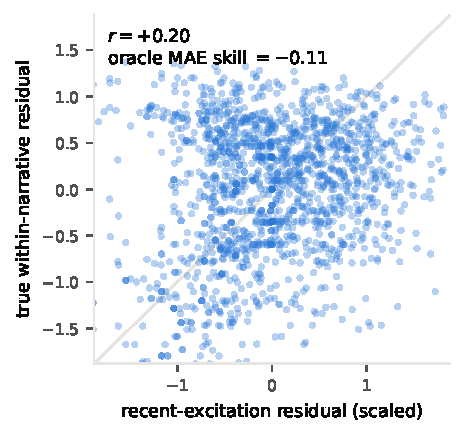
\includegraphics[width=0.9\linewidth]{figures/oracle_noise.pdf}
\caption{\textbf{The negative result, visualised.} True within-narrative
engagement residual vs.\ the (scaled) residual of the leak-free
recent-excitation feature --- the strongest causal predictor available to any
model. A real but weak rank signal exists ($r = +0.20$), yet the Poisson-scale
cloud dominates: an oracle regressor built on this feature has \emph{negative}
MAE skill ($-0.11$) against a narrative-mean predictor. Engagement magnitude
is not a usable headline metric under near-critical cascade dynamics.}
\label{fig:oracle}
\end{figure}

\paragraph{(1) Engagement magnitude is intrinsically noise-dominated --- a
negative result (\cref{fig:oracle}).} On log-engagement regression, no model (including ours)
beats the naive train-mean (MAE 0.825 vs.\ SimCity 0.848). We show this is a
property of the target, not the models: an \emph{oracle} ridge regressor handed
a leak-free recent-excitation feature achieves \emph{negative} within-narrative
residual skill ($-0.107$) and near-random surge-ranking AUC (0.507), because
next-window branching-process counts carry Poisson-scale variance. We therefore
argue engagement-magnitude regression is an ill-posed headline metric for
cascade models, and evaluate timing and transfer instead.

\paragraph{(2) Cross-platform next-event timing --- a null result.} Using the
conditional intensity $\lambda_i(t_k)$ (causal, history strictly before $t_k$)
to predict which platform fires next, SimCity attains AUC
$0.610 \pm 0.005$ vs.\ static MHP $0.605 \pm 0.000$ over three seeds. Although
SimCity is nominally ahead on every seed, the margin is \emph{not}
statistically significant (Welch $p = 0.23$) and we report it as a null
result: on this task the neural conditioning does not demonstrably improve on
a global Hawkes parameterisation. The temporal machinery is nonetheless
functioning --- shuffling test timestamps inflates SimCity's Hawkes NLL by
$15$--$25\times$ --- but next-event platform identity is largely determined by
platform autocorrelation (a last-platform persistence rule reaches 0.982
accuracy on the real corpus), leaving little headroom for any model.

\paragraph{(3) Narrative transfer detection --- the headline result
(\cref{fig:transfer}, \cref{tab:transfer}).} We ask:
among narratives so far observed on a \emph{single} platform, which will later
jump platforms? SimCity's per-narrative mean off-diagonal branching mass
$\sum_{i \ne j} \hat\alpha_{ij}/\hat\gamma_{ij}$ (``bridge score''), computed
causally from pre-switch events only, ranks 209 test narratives (123 transfer)
with \textbf{AUC $0.653 \pm 0.005$ over three seeds} (per-seed 0.649/0.658/0.652;
95\% bootstrap CI $[0.58, 0.73]$; Mann--Whitney $p < 1.1\times10^{-4}$ on every
seed). The score survives confound controls on all seeds: AUC 0.656--0.662
within event-count strata and 0.656--0.661 within latent-reach strata, versus
0.551 for the popularity baseline. A static MHP has a single global $\alpha$ and cannot rank narratives at all
(AUC 0.5 by construction), but beating a baseline that is degenerate by
construction establishes little. The load-bearing comparator is therefore a
\emph{per-narrative} Hawkes process: independent MLE fits, no graph
conditioning. Because a pre-switch window contains events on a single platform
by construction, such a fit cannot identify cross-platform $\alpha_{ij}$ at
all; it can only characterise the narrative's own arrival dynamics, from a
median of three events. Granting it one validation-selected degree of freedom
(statistic and sign), matching SimCity's, it reaches AUC 0.63 on the synthetic
benchmark versus SimCity's 0.65, with paired-bootstrap intervals excluding zero
on two of three seeds (\cref{tab:transfer}). The gap is the value of
\emph{amortisation}: the neural head learns a shared map from narrative state
to excitation parameters across all narratives, where independent fitting has
only each narrative's handful of events (median three).

\paragraph{Delimiting the claim: a non-Hawkes benchmark.} To test whether this
capability reflects transfer \emph{per se} or transfer specifically mediated by
temporal excitation, we build a second benchmark from a structurally different
mechanism: narratives spread by SIR contagion over a multiplex social graph,
and cross-platform transfer occurs \emph{topologically} --- when the contagion
reaches a bridge user present on both platforms who cross-posts --- with no
excitation kernel anywhere in the generator. Here the bridge score is at chance
(AUC $0.46 \pm 0.10$ over three seeds). The method therefore detects transfer
that is \emph{temporally excited}, not transfer in general --- a distinction
that turns out to be decisive on real data (paragraph (4)).

\paragraph{(4) On real data, transfer is not temporally excited --- and a
cautionary tale.} We evaluate on a live Hacker News + GDELT corpus (32{,}472
events, 40/60 platform split) with narratives formed by sentence-embedding
clustering of story and article titles. On this corpus the bridge score is at
chance: oriented per-seed AUCs 0.532 / 0.497 / 0.511 (\textbf{$0.51 \pm 0.02$}
over three seeds; none significant, Mann--Whitney $p = 0.15/0.54/0.36$), while
the \emph{popularity} baseline predicts transfer well (AUC 0.65). The result is
not underpowered: with 85 positives among 4{,}904 test narratives the seed
spread is tight ($\pm 0.02$), and the popularity baseline succeeding on the same
data shows the task carries learnable signal that the excitation score does not
capture. Together with the SIR benchmark, this indicates that real HN\,$\to$\,news
transfer is popularity- and topology-driven rather than temporally excited ---
exactly the regime in which \cref{sec:results}(3) predicts our method should
fail.

\paragraph{(5) What does predict real transfer
(\cref{fig:real-pred}, \cref{tab:real-pred}).} That the neural score fails does
not mean transfer is unpredictable. We fit a logistic-regression classifier on
eight interpretable features computed causally from each narrative's
single-platform (pre-switch) window --- volume, rate, duration, burstiness,
source diversity, mean/max engagement, and exogenous-volume proxy --- and
evaluate by stratified 5-fold cross-validation. The full model reaches
\textbf{ROC-AUC $0.82 \pm 0.05$}, and the signal is concentrated in
\emph{engagement}: mean and max log-engagement each reach $\approx 0.81$ as
\emph{single} features, whereas raw popularity (event count) reaches only
$0.65$ and burstiness/timing features barely exceed chance. Real narratives
cross platforms when they attract engagement early, essentially independent of
how their events cluster in time --- the opposite of what a temporal-excitation
model keys on, which is precisely why the neural score is at chance here while a
one-feature engagement model is not. This is a strong, reproducible, and
interpretable baseline for cross-platform transfer prediction, and it locates
the phenomenon empirically: transfer is attention-driven, not
excitation-driven.

\paragraph{A cautionary result.} We reached the negative neural finding by
correcting our own error. An earlier version of this corpus reported AUC
$0.78 \pm 0.10$. Following the reviewer-style protocol of \emph{sampling our own
clusters and reading them}, we found a defect in our greedy clusterer --- once a
cluster-count cap was hit, remaining items were assigned to their nearest
centroid \emph{regardless of similarity} --- which had merged unrelated HN
stories and news articles into single ``narratives'' (only 2--3\% of
cross-source pairs exceeded a 0.5 title-embedding cosine). The $0.78$ was
measured over these spurious narratives. With the clusterer corrected (no forced
assignment; time-windowed clusters) the neural effect disappears while the
engagement result above holds. We adjudicated a random sample of 60 cross-source
cluster pairs by reading the paired titles (labels released): 62\% are the same
news event, rising to 80\% for pairs above 0.65 cosine. This residual cluster
noise only \emph{attenuates} measured predictability --- a spurious merge
injects a false transfer label uncorrelated with the narrative's real
engagement --- so the engagement AUC of 0.82 is a lower bound on the true
signal. The synthetic results are unaffected, as narrative identity there is
ground truth by construction. We report this in full because it is the kind of
failure that peer review rarely catches but reproducibility should.

\begin{figure}[t]
\centering
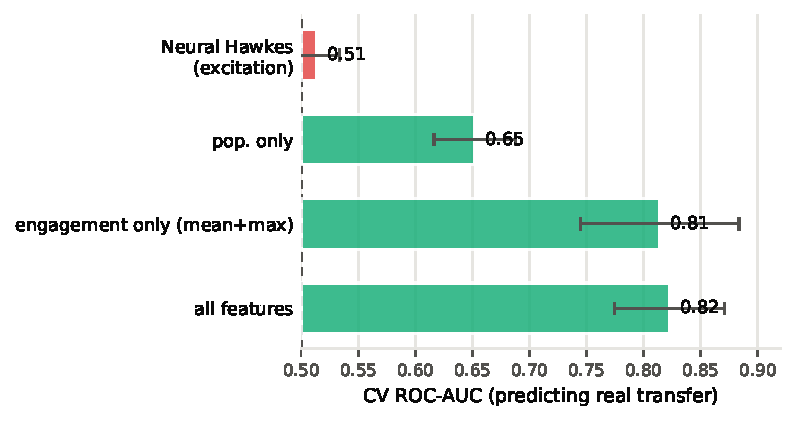
\includegraphics[width=\linewidth]{figures/real_predictors.pdf}\\[4pt]
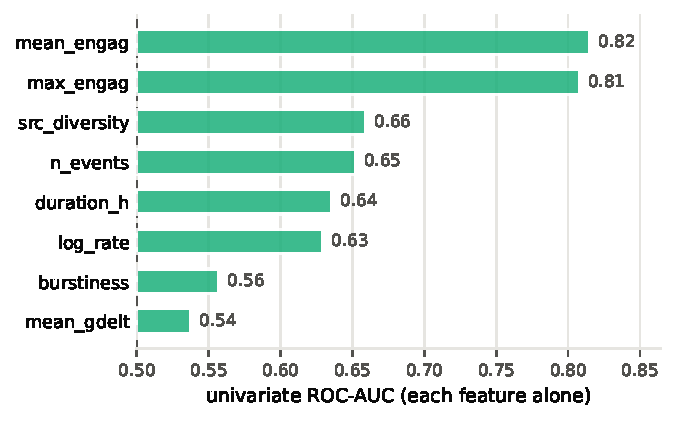
\includegraphics[width=\linewidth]{figures/real_coefficients.pdf}
\caption{\textbf{What predicts real cross-platform transfer.} \emph{Top:}
5-fold CV ROC-AUC. The neural excitation score is at chance; interpretable
single-platform features reach 0.82. \emph{Bottom:} univariate ROC-AUC per
feature (each alone). Early engagement is the dominant signal ($\approx 0.81$);
raw volume and timing/burstiness features are far weaker. Transfer is
attention-driven, not excitation-driven.}
\label{fig:real-pred}
\end{figure}

\begin{table}[t]
\centering
\small
\caption{\textbf{Predicting real transfer} (corrected corpus; 4{,}904 test
narratives, 85 transfer; stratified 5-fold CV).}
\label{tab:real-pred}
\begin{tabular}{lc}
\toprule
\textbf{Predictor} & \textbf{CV ROC-AUC} \\
\midrule
SimCity bridge score (neural Hawkes) & $0.51$ (chance) \\
Popularity only (event count)        & $0.65 \pm 0.04$ \\
Engagement only (mean, max)          & $0.81 \pm 0.07$ \\
All interpretable features           & $\mathbf{0.82 \pm 0.05}$ \\
\bottomrule
\end{tabular}
\end{table}

\subsection{Limitations and Negative Results}
\label{sec:limitations}

We report the following limitations. (0) \textbf{Only two of the six
architectural components are empirically load-bearing.} The TGN core and the
cross-platform Hawkes head carry every result reported here; the SEIR-Z-D
compartmental layer, the HMF bridge, the smooth Deffuant dynamics, and the
dynamic influence score are \emph{specified and released as a simulation
layer but not independently validated} in this paper. We flag this explicitly
rather than letting the breadth of the framework imply otherwise. (i) The multi-task
objective interacts with the \emph{timing} metric: with uniform Kendall
weighting the neural model underperforms the static MHP on next-event timing
(AUC 0.576), recovered by up-weighting the Hawkes task. Importantly, a
loss-weight sweep ($\{1,3,10,30\}\times$) shows the \emph{transfer} AUC --- our
headline --- is essentially flat (0.63--0.66), so the central result is not an
artifact of this weighting; only the (null) timing result is weight-sensitive. (ii) Our method predicts only
temporally-excited transfer; on the real corpus, where transfer is
popularity-driven, it is at chance, so it is not a general-purpose transfer
detector (\cref{sec:results}(3),(4)). (iii) The timing margin over static MHP,
while consistent across seeds, is small and not significant. (iv) Results are
on a two-platform real corpus (HN + news); the third social platform (Reddit/X)
remains future work pending API access. (v) Real-corpus narratives are formed
by embedding clustering of titles; a read-and-adjudicate sample of 60
cross-source pairs gives 62\% same-event precision (80\% above 0.65 cosine),
with the residual noise attenuating rather than inflating our predictability
estimates. Our adjudication was performed with LLM assistance and released for
verification; a fully human-labelled figure would be stronger. This limitation
is also the source of our cautionary result: an earlier greedy clusterer with a
forced-assignment defect inflated the real transfer AUC to $0.78$ before we
caught it by sampling our own clusters.

\subsection{Reproducibility}
All experiments run on CPU. The repository releases the generator, collectors,
training (\texttt{train.py} with seed and task-weight environment controls),
and one-command evaluations (\texttt{multiseed\_stats.py},
\texttt{narrative\_transfer\_eval.py}, \texttt{platform\_prediction\_eval.py},
\texttt{burst\_ranking\_eval.py}, oracle checks), with all tables regenerable
from \texttt{results/}.

% =============================================================
% Bibliography
% =============================================================
\bibliography{references}

\appendix

\section*{Appendix A: Notation Reference}

\begin{center}
\small
\setlength{\tabcolsep}{4pt}
\begin{tabular}{ll}
\toprule
\textbf{Symbol} & \textbf{Meaning} \\
\midrule
$\bn(t)$ & State vector $(n_S,n_E,n_I,n_R,n_Z,n_D)$ \\
$\br_k$ & Jump vector for transition $k$ \\
$\beta(t)$ & Macroscopic SEIR-Z exposure rate \\
$\hat{\beta}_{v,c}(t)$ & TGN node-level predicted infectivity \\
$\hat{\alpha}_{ij}(t)$ & Neural Hawkes infectivity (platform $j\to i$) \\
$\hat{\gamma}_{ij}(t)$ & Neural Hawkes decay parameter \\
$\gamma_I$ & SEIR Infected-to-Recovered decay rate \\
$\sigma$ & SEIR Exposed-to-Infected activation rate \\
$\eta$ & Deffuant opinion convergence rate \\
$\zeta(t)$ & Zombie resurgence rate (Hawkes-coupled) \\
$\delta_D$ & Archival rate ($Z\to D$) \\
$\theta$ & Algorithmic boost factor for Zombie content \\
$\epsilon_p(v)$ & Platform-specific confidence bound \\
$\rho$ & Deffuant smoothing steepness \\
$\tau$ & Platform pooling temperature \\
$P(k'|k)$ & Degree-degree conditional distribution \\
$k_v(t)$ & Effective temporal degree (\cref{eq:temporal-degree}) \\
$I(v,t)$ & Dynamic influence score \\
$\hv_{\cP_i}(t)$ & Platform-level pooled embedding \\
$\mu_i(t)$ & Hawkes exogenous background rate (GDELT) \\
$|\cP|$ & Number of platforms \\
$\cP_i$ & Set of nodes on platform $i$ \\
\bottomrule
\end{tabular}
\end{center}

\section*{Appendix B: Deffuant $\rho$ Sensitivity Analysis}

The smooth formulation (\cref{eq:deffuant}) recovers the hard-threshold model
as $\rho \to \infty$; we conjecture cluster invariance for $\rho > 10^2$, with
a systematic sweep left as future work. No result in \cref{sec:results}
depends on $\rho$.

\end{document}